\documentclass[10.5pt,a4paper]{article}
\usepackage[margin=1.9cm,top=2.1cm,bottom=1.9cm]{geometry}
\usepackage[T1]{fontenc}
\usepackage{lmodern}
\usepackage{amsmath,amssymb}
\usepackage{enumitem}
\usepackage{booktabs,array,multirow}
\usepackage{xcolor}
\usepackage{fancyhdr}
\usepackage[most]{tcolorbox}
\usepackage{tikz}
\usetikzlibrary{automata,positioning,arrows.meta,calc}
\usepackage[hidelinks,pdftitle={CSE 211 Final Study Guide}]{hyperref}

\definecolor{navy}{HTML}{1F3864}
\definecolor{recbg}{HTML}{EEF3FA}
\definecolor{qbg}{HTML}{F6F6F6}
\definecolor{exbg}{HTML}{F4FAF4}
\definecolor{exborder}{HTML}{2E7D32}
\definecolor{trapbg}{HTML}{FDF0F0}
\definecolor{trapborder}{HTML}{C62828}

\setlist{itemsep=1pt,topsep=3pt,parsep=0pt,leftmargin=1.5em}
\setlength{\parindent}{0pt}
\setlength{\parskip}{4pt}
\renewcommand{\arraystretch}{1.15}

\pagestyle{fancy}
\fancyhf{}
\lhead{\small\color{gray}CSE 211 --- Final study guide}
\rhead{\small\color{gray}\leftmark}
\cfoot{\small\color{gray}\thepage}
\renewcommand{\headrulewidth}{0.3pt}

% recipe box
\newtcolorbox{recipe}[1][]{breakable,colback=recbg,colframe=navy,boxrule=0.4pt,leftrule=3pt,arc=1pt,
  left=6pt,right=6pt,top=4pt,bottom=4pt,title={#1},fonttitle=\bfseries\small,coltitle=white,colbacktitle=navy,before skip=6pt}
% exam question (upper) + written answer (lower)
\newtcolorbox{examq}[2]{breakable,enhanced,colback=qbg,colbacklower=exbg,colframe=exborder,boxrule=0.5pt,leftrule=3pt,arc=1pt,
  left=7pt,right=7pt,top=4pt,bottom=4pt,title={Exam answer --- #1 \hfill (#2)},fonttitle=\bfseries\small,coltitle=white,
  colbacktitle=exborder,segmentation style={solid,exborder,line width=0.4pt},before skip=8pt,fontupper=\itshape}
\newtcolorbox{trap}{breakable,colback=trapbg,colframe=trapborder,boxrule=0.4pt,leftrule=3pt,arc=1pt,
  left=6pt,right=6pt,top=3pt,bottom=3pt,before skip=6pt}
\newcommand{\TRAP}{\textbf{\color{trapborder}Trap.\ }}
\newcommand{\asked}[1]{{\small\color{gray!60!black}\textbf{What they ask:} #1}\par}
\newcommand{\ansh}[1]{\textbf{\color{exborder}#1}\ }

\tikzset{every state/.style={minimum size=0.8cm,inner sep=1pt,font=\small},
  >={Stealth[length=2mm]},auto,node distance=2.1cm,every edge/.append style={font=\small}}

\newcommand{\Sig}{\Sigma}
\newcommand{\eps}{\varepsilon}
\newcommand{\NP}{\mathrm{NP}}
\renewcommand{\P}{\mathrm{P}}
\newcommand{\PS}{\mathrm{PSPACE}}

\begin{document}

% ------------------------------------------------------------------ title
\begin{center}
{\Large\bfseries\color{navy} CSE 211 --- Theory of Computation}\\[2pt]
{\large Final study guide: the method for every question type, with past-paper questions answered as you would write them}\\[2pt]
{\small Part A: Hakim Sir (Topics 1--6) \quad$\cdot$\quad Part B: Atif Sir (Topics 7--12)\quad$\cdot$\quad Term final: 10 November 2026}
\end{center}

\begin{tcolorbox}[colback=white,colframe=navy,boxrule=0.4pt,arc=1pt,left=6pt,right=6pt,top=3pt,bottom=3pt]
\textbf{How this guide is built.} Every topic opens with \emph{what they ask} (counted from the practice-tracker papers, 2017-18 to 2023-24),
then a blue \emph{recipe}, then green \emph{exam answers}: a real past question in the grey upper half and, below the line, the answer written the
way it should appear in your script --- design idea, construction, table or diagram, a check, and a closing sentence. Red boxes are the mistakes
that lose marks.\\[2pt]
\textbf{Companions.} Full proofs: \texttt{CSE211\_Proofs\_Exam\_Ready.pdf}. Every tracker question with a solution:
\texttt{CSE211\_Hakim/Atif\_TF\_Questions\_Solutions.pdf}.\\[2pt]
\textbf{Checked by program} (\texttt{\_build/verify\_guide\_v2.py}, \texttt{\_build/verify\_final\_guide.py}): every DFA, NFA, regular expression,
grammar, CYK table, PDA and Turing machine in the exam answers, on all strings up to length 7--12.
\end{tcolorbox}

\begin{recipe}[How to write any answer for full marks]
\begin{enumerate}
\item \textbf{Idea first, in one or two sentences} (``the state remembers \dots'', ``the stack holds one $A$ per $a$ \dots''). Several questions
say rules alone get no marks.
\item \textbf{Name every state / variable / stack symbol and say what it means.} Mark start ($\to$) and accepting ($*$ or double circle) states.
\item \textbf{Give the full object:} diagram \emph{and} table when asked; every DFA state has a move on every symbol (dead state).
\item \textbf{Check on the string the question names and on one string that must fail}; show the trace (states, IDs, CYK table, tape).
\item \textbf{End with one sentence that answers the question} (``Hence $0100\in L(G)$'', ``So $L$ is not regular'').
\item \textbf{Time:} roughly 1.5 minutes per mark; a 15-mark design question is about 20 minutes. Do the design and the trace before polishing.
\end{enumerate}
\end{recipe}

\begin{center}\small
\begin{tabular}{@{}llc>{\raggedright\arraybackslash}p{10.6cm}@{}}
\toprule
& Topic & Tracker Qs & The question that keeps coming back\\\midrule
\multirow{6}{*}{\rotatebox{90}{Hakim}} & 1 Introduction & 4 & ``which area of ToC / why hard problems are useful'' (Q1(a), 4--15 marks)\\
& 2 DFA & 13 & design a DFA (counter, mod-$m$, forbidden substring); describe a DFA's language\\
& 3 NFA & 13 & design an NFA; $\eps$-NFA $\to$ DFA; strings of length $\le3$ accepted\\
& 4 Regular languages & 24 & closure constructions with $\delta$; choose/design/simplify regular expressions; RE $\to$ NFA\\
& 5 Pumping lemma & 9 & prove non-regular; ``what is wrong with Skye's/BLP's argument''\\
& 6 CFG & 15 & design a CFG (with design idea); show a grammar is ambiguous\\\midrule
\multirow{6}{*}{\rotatebox{90}{Atif}} & 7 CNF and CYK & 7 & CYK on a CNF grammar (5 papers); CNF conversion (2)\\
& 8 PDA, CFL pumping & 10 & design a PDA with diagram (every paper); final state = empty stack; non-CFL proof\\
& 9 TM design & 6 & TM on tape $w_1cw_2c$: AND / OR / XOR / equality / NOT / 2's complement (every paper)\\
& 10 TM variants & 6 & one-tape TM simulates multitape; true/false on simulations (every paper)\\
& 11 Undecidability & 7 & $L_d$ not RE, or halting problem RE but not recursive (every paper)\\
& 12 Complexity & 17 & Cook's theorem clause (4 papers), Venn diagram / PSPACE $=$ NPSPACE (every paper), NP-completeness\\\bottomrule
\end{tabular}
\end{center}

\tableofcontents

% ================================================================== PART A
\clearpage
\section*{Part A --- Hakim Sir}\addcontentsline{toc}{section}{Part A --- Hakim Sir}

% ------------------------------------------------------------------ 1
\section{Introduction: what Theory of Computation is for}\markboth{1 Introduction}{}
\asked{2023-24 Q1(a), 2022-23 Q1(a), 2021-22 Q1(a), 2019-20 Q1(b): short essay answers, 4--15 marks.}
\begin{recipe}[Recipe --- ``which area / why hard problems'' questions]
\begin{enumerate}
\item Name the three central areas: \textbf{automata} (what can be done with limited memory), \textbf{computability} (what can be solved at
all), \textbf{complexity} (what can be solved efficiently).
\item Say what the system must \emph{do} and match it: bounded-memory pattern checking $\to$ automata (DFA); ``does any algorithm exist''
$\to$ computability; ``how much time / is it infeasible'' $\to$ complexity.
\item Give the concrete model or class, and the consequence (hardness is \emph{useful} for security).
\end{enumerate}
\end{recipe}

\begin{examq}{2021-22 Q1(a)}{4 marks}
In the password-protected login system of a computer, which of the three traditionally central areas of the Theory of Computation has been
applied? Explain clearly.
\tcblower
\ansh{Answer.} Two areas are applied.\\
\emph{Automata theory} --- checking that a new password obeys the rules (e.g.\ at least 8 characters, a digit, an upper-case letter) needs only
a bounded memory of the prefix read: $\min(\text{length},8)$, ``digit seen'', ``upper case seen''. So the set of valid passwords is a regular
language and is checked by a DFA in one left-to-right pass.\\
\emph{Complexity theory} --- the system stores $h(\text{password})$ for a one-way hash $h$. Computing $h$ is easy (polynomial time), but finding
a password with a given hash is believed infeasible. Security rests on this gap between easy and hard.\\
Computability plays no role: every task here is decidable.
\end{examq}

\begin{examq}{2022-23 Q1(a) and 2019-20 Q1(b)}{10 / 15 marks}
Explain public and private keys in asymmetric cryptography and the role of ToC; describe a scenario that specifically needs computationally
hard problems.
\tcblower
\ansh{Answer.} In asymmetric cryptography each user has a \emph{public key} (published, used to encrypt or to verify signatures) and a
\emph{private key} (kept secret, used to decrypt or to sign). In RSA the public key contains $n=pq$ and the private key needs $p,q$.\\
\emph{Role of ToC (complexity).} Encryption with the public key is easy (polynomial time). Decrypting without the private key amounts to
factoring $n$, for which no polynomial-time algorithm is known. A proposed key is easy to \emph{check} (multiply $p\cdot q$) but hard to
\emph{find} --- the same ``verify easy / find hard'' gap as $\NP$ versus $\P$. If $\P=\NP$, such schemes would collapse.\\
\emph{Scenario that needs hard problems:} online banking / HTTPS key exchange, digital signatures, password hashing, CAPTCHAs and
proof-of-work. Here hardness is a \emph{resource}: the system is safe exactly because the attacker's problem is hard.
\end{examq}

\begin{examq}{2023-24 Q1(a)}{8 marks}
What options do we have when a problem appears to be computationally hard?
\tcblower
\ansh{Answer.} (1) \emph{Prove it hard} (NP-complete) so we stop looking for an exact fast algorithm. (2) \emph{Approximation}: a
polynomial algorithm with a guaranteed ratio (e.g.\ vertex cover within factor 2). (3) \emph{Heuristics / local search}: good answers fast,
no guarantee. (4) \emph{Special cases}: restrict the input (trees, bounded degree, 2-SAT is in $\P$). (5) \emph{Exact exponential algorithms}
for small inputs (backtracking, branch and bound, dynamic programming). (6) \emph{Randomisation} and average-case analysis. (7) Use the
hardness: cryptography.
\end{examq}

% ------------------------------------------------------------------ 2
\section{DFA design}\markboth{2 DFA design}{}
\asked{13 questions. Design (2023-24 Q1(b), Q2(b); 2022-23 Q1(c), Q3(a); 2021-22 Q1(b); 2019-20 Q1(c), Q2(c); 2017-18 Q2(b)); describe the
language of a given DFA (2022-23 Q2(a), 2020 Q2(a)); theory (role of a state, accepting states and the table).}
\begin{recipe}[Recipe --- designing a DFA]
\begin{enumerate}
\item Ask \emph{what is the least I must remember about the prefix read so far?} Each possible value is a state. Typical memories: a count
capped at $k$, a remainder mod $m$, the last one or two symbols, a phase, ``already failed'' (dead state).
\item Start state = memory of $\eps$. Accepting states = memory values meaning ``accept''.
\item Fill $\delta$ for \emph{every} (state, symbol) pair; send impossible continuations to one dead state.
\item Draw the diagram, write the table if asked, test the named strings, $\eps$, and one rejected string.
\end{enumerate}
\textbf{Numbers in base $b$ mod $m$:} digit $d$ turns value $v$ into $bv+d$, so $\delta(r,d)=(br+d)\bmod m$.
\textbf{Running sum with reset $R$:} $\delta(r,d)=(r+d)\bmod m$, $\delta(r,R)=0$.
\end{recipe}

\begin{examq}{2021-22 Q1(b)}{10 marks}
Design a DFA with not more than five states for $\Sigma=\{a,b\}$ which accepts the strings that begin with $a$ but do not contain the substring
$aab$. Showing only the state diagram should suffice.
\tcblower
\ansh{Design idea.} The first symbol must be $a$ (a first $b$ goes to a dead state). After that, $aab$ appears exactly when a $b$ is read while
the input ends in $aa$, so it is enough to remember whether the input ends in $b$, in a single $a$, or in $aa$.\\
\ansh{States.} $q_0$: nothing read. $A$: ends in a single $a$. $AA$: ends in $aa$. $B$: ends in $b$ (the start was fine). $d$: dead (began
with $b$, or $aab$ seen). Accepting: $A,AA,B$. Five states.
\begin{center}
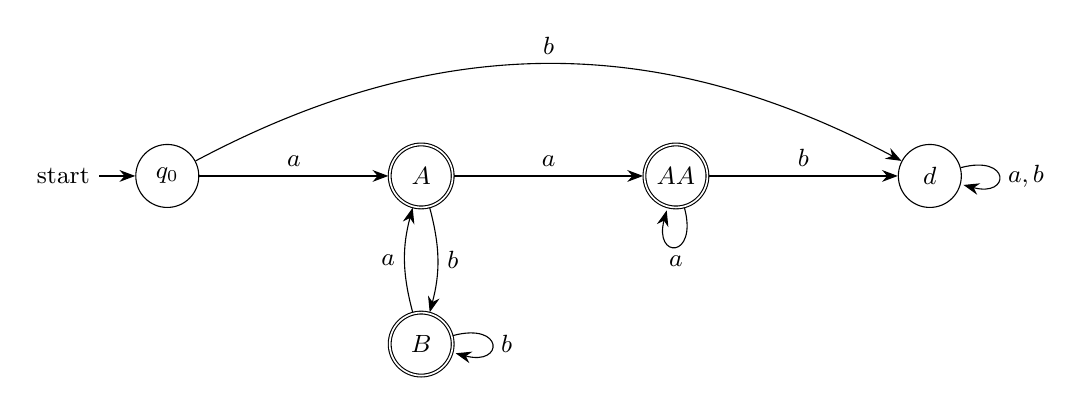
\begin{tikzpicture}[node distance=2.4cm]
\node[state,initial] (q0) {$q_0$};
\node[state,accepting,right=of q0] (A) {$A$};
\node[state,accepting,right=of A] (AA) {$AA$};
\node[state,right=of AA] (d) {$d$};
\node[state,accepting,below=1.3cm of A] (B) {$B$};
\path[->] (q0) edge node {$a$} (A)
 (q0) edge[bend left=28] node {$b$} (d)
 (A) edge node {$a$} (AA)
 (A) edge[bend left=15] node {$b$} (B)
 (B) edge[bend left=15] node {$a$} (A)
 (B) edge[loop right] node {$b$} ()
 (AA) edge[loop below] node {$a$} ()
 (AA) edge node {$b$} (d)
 (d) edge[loop right] node {$a,b$} ();
\end{tikzpicture}
\end{center}
\ansh{Check.} $abab$: $q_0\to A\to B\to A\to B$ accept. $aaab$: $q_0\to A\to AA\to AA\xrightarrow{b}d$ reject (contains $aab$).
$ba$: $q_0\xrightarrow{b}d$ reject. $aaa$: ends in $AA$, accept. Hence the DFA accepts exactly the required language.
\end{examq}

\begin{examq}{2019-20 Q1(c)}{15 marks}
Draw a DFA over $\{0,1,2,R\}$ that keeps the running sum of the digits, resetting it to 0 on $R$; accept if the sum is 1 or 2 modulo 5.
\tcblower
\ansh{Design idea.} Only the sum mod 5 matters, so five states $s_0,\dots,s_4$ ($s_i$: sum $\equiv i$). Digit $d$: $s_i\to s_{(i+d)\bmod5}$;
$R$: every state $\to s_0$. Start $s_0$; accepting $s_1,s_2$.
\begin{center}\small
\begin{tabular}{c|cccc}
 & 0 & 1 & 2 & $R$\\\hline
$\to s_0$ & $s_0$ & $s_1$ & $s_2$ & $s_0$\\
$*s_1$ & $s_1$ & $s_2$ & $s_3$ & $s_0$\\
$*s_2$ & $s_2$ & $s_3$ & $s_4$ & $s_0$\\
$s_3$ & $s_3$ & $s_4$ & $s_0$ & $s_0$\\
$s_4$ & $s_4$ & $s_0$ & $s_1$ & $s_0$
\end{tabular}
\end{center}
(Draw the five states in a ring: each 0 is a self-loop, 1 goes one step round, 2 goes two steps round, every $R$ returns to $s_0$.)
\ansh{Check.} $12R2$: $s_0\to s_1\to s_3\xrightarrow{R}s_0\to s_2$ accept (sum after reset is 2). $22$: $s_0\to s_2\to s_4$ reject (sum 4).
\end{examq}

\begin{trap}\TRAP Every state needs an arrow for every symbol --- draw the dead state. Accept $\eps$ only if the language contains it.
For ``binary multiple of $m$ beginning with 1'' add a separate start state (a leading 0 goes to dead).
\textbf{Theory answers:} a state is a \emph{summary of everything relevant about the input read so far} (finite memory); accepting states do
\emph{not} change the rows or columns of the transition table (rows = states, columns = symbols), they are only marked with $*$.
\textbf{2022-23 Q1(b):} a 2-state DFA (``remainder 0 / non-zero'') cannot track a sum mod 3: after ``1'' and after ``2'' it would be in the
same state, yet appending ``2'' gives sums 3 (remainder 0) and 4 (remainder 1). Strings that must be told apart need different states.\end{trap}

% ------------------------------------------------------------------ 3
\section{NFA, $\varepsilon$-moves and subset construction}\markboth{3 NFA and subset construction}{}
\asked{13 questions. Design an NFA (2023-24 Q3(a), Q4(a); 2022-23 Q4(b); 2021-22 Q3(b); 2019-20 Q3(b); 2017-18 Q3(a)); convert an $\eps$-NFA
to a DFA (2021-22 Q3(c), 2020 Q4(b), 2017-18 Q4(a)); list accepted strings of length $\le3$ (2020 Q1(c)).}
\begin{recipe}[Recipe --- NFA design and NFA $\to$ DFA]
\textbf{Design:} let the NFA \emph{guess} the moment something happens (``the suffix starts here''); for ``$X$ or $Y$'' build two small
machines and join them with $\eps$-edges from a new start state.\\
\textbf{$\eps$-NFA $\to$ DFA (subset construction):}
\begin{enumerate}
\item Write $E(q)$, the $\eps$-closure of every state. DFA start state $=E(q_0)$.
\item For each new subset $S$ and symbol $a$: $\delta_D(S,a)=E\big(\bigcup_{q\in S}\delta(q,a)\big)$. Keep going until no new subset appears.
\item Only \emph{reachable} subsets; $\emptyset$ is the dead state. Accepting = subsets containing an accepting NFA state.
\item Show the table, then draw the DFA.
\end{enumerate}
\end{recipe}

\begin{examq}{2021-22 Q3(c)}{9 marks}
Convert the following NFA into an equivalent DFA (start $q_1$, accepting $q_2$):\quad
$q_1$: $a\to\{q_3\}$, $\eps\to\{q_2\}$;\quad $q_2$: $a\to\{q_1\}$;\quad $q_3$: $a\to\{q_2\}$, $b\to\{q_2,q_3\}$.
\tcblower
\ansh{$\eps$-closures.} $E(q_1)=\{q_1,q_2\}$, $E(q_2)=\{q_2\}$, $E(q_3)=\{q_3\}$. DFA start state $=E(q_1)=\{q_1,q_2\}$.\\
\ansh{Subset table.}
\begin{center}\small
\begin{tabular}{l|l|l}
DFA state & on $a$ & on $b$\\\hline
$\to *\{q_1,q_2\}$ & $E(\{q_3\}\cup\{q_1\})=\{q_1,q_2,q_3\}$ & $\emptyset$\\
$*\{q_1,q_2,q_3\}$ & $E(\{q_3,q_1,q_2\})=\{q_1,q_2,q_3\}$ & $E(\{q_2,q_3\})=\{q_2,q_3\}$\\
$*\{q_2,q_3\}$ & $E(\{q_1,q_2\})=\{q_1,q_2\}$ & $E(\{q_2,q_3\})=\{q_2,q_3\}$\\
$\emptyset$ (dead) & $\emptyset$ & $\emptyset$
\end{tabular}
\end{center}
Accepting: every subset containing $q_2$, i.e.\ the three non-empty ones. Four reachable states out of $2^3=8$.
\begin{center}
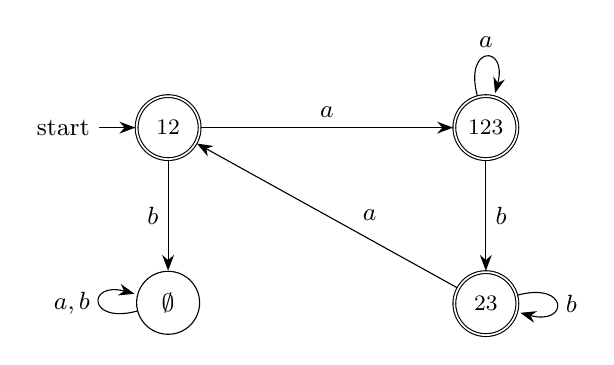
\begin{tikzpicture}[node distance=3.2cm]
\node[state,initial,accepting] (a) {\footnotesize$12$};
\node[state,accepting,right=of a] (b) {\footnotesize$123$};
\node[state,accepting,below=1.4cm of b] (c) {\footnotesize$23$};
\node[state,below=1.4cm of a] (z) {$\emptyset$};
\path[->] (a) edge node {$a$} (b) (a) edge node[swap] {$b$} (z)
 (b) edge[loop above] node {$a$} () (b) edge node {$b$} (c)
 (c) edge node[swap,pos=0.4] {$a$} (a) (c) edge[loop right] node {$b$} ()
 (z) edge[loop left] node {$a,b$} ();
\end{tikzpicture}
\end{center}
\ansh{Check.} $\eps$: accepted in the NFA ($q_1\xrightarrow{\eps}q_2$) and in the DFA (start is accepting). $b$: the NFA has no $b$-move from
$q_1,q_2$, the DFA goes to $\emptyset$: both reject. So the DFA is equivalent to the NFA.
\end{examq}

\begin{examq}{2021-22 Q3(b)}{10 marks}
Design an NFA which accepts binary strings containing at least two 0s, or exactly two 1s. Showing only the state diagram should suffice.
\tcblower
\ansh{Design idea.} Union of two counters: a new start state $s$ guesses with $\eps$-edges which condition will hold. Upper branch counts 0s
up to 2 (1s are ignored); lower branch counts 1s and has \emph{no} move on a third 1, so that branch dies.
\begin{center}
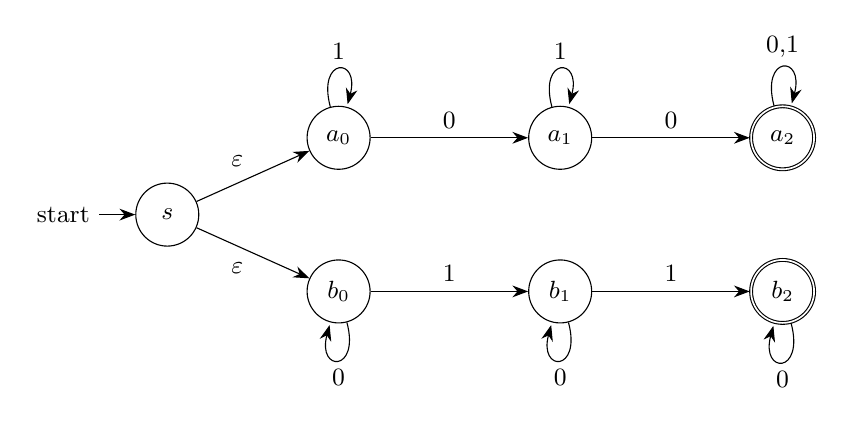
\begin{tikzpicture}[node distance=2cm]
\node[state,initial] (s) {$s$};
\node[state,above right=0.4cm and 1.6cm of s] (a0) {$a_0$};
\node[state,right=of a0] (a1) {$a_1$};
\node[state,accepting,right=of a1] (a2) {$a_2$};
\node[state,below right=0.4cm and 1.6cm of s] (b0) {$b_0$};
\node[state,right=of b0] (b1) {$b_1$};
\node[state,accepting,right=of b1] (b2) {$b_2$};
\path[->] (s) edge node {$\eps$} (a0) (s) edge node[swap] {$\eps$} (b0)
 (a0) edge node {0} (a1) (a1) edge node {0} (a2)
 (a0) edge[loop above] node {1} () (a1) edge[loop above] node {1} () (a2) edge[loop above] node {0,1} ()
 (b0) edge node {1} (b1) (b1) edge node {1} (b2)
 (b0) edge[loop below] node {0} () (b1) edge[loop below] node {0} () (b2) edge[loop below] node {0} ();
\end{tikzpicture}
\end{center}
\ansh{Check.} $0110$: upper branch reaches $a_2$ (two 0s) --- accept. $1011$: one 0, three 1s; upper ends in $a_1$, lower dies on the
third 1 --- reject. $101$: lower ends in $b_2$ --- accept.
\end{examq}

\begin{trap}\TRAP Never list all $2^n$ subsets --- only reachable ones. Take the $\eps$-closure at the start \emph{and} after every move.
``Accepted strings of length $\le3$'' (2020 Q1(c)): follow every branch for each length 0, 1, 2, 3 and write the general form
(e.g.\ ``any string ending in $c$''). A 5-state NFA gives a DFA with between 1 and $2^5=32$ states.\end{trap}

% ------------------------------------------------------------------ 4
\section{Regular languages: closure, regular expressions, state elimination}\markboth{4 Regular languages}{}
\asked{24 questions --- the biggest topic. Closure constructions with $\delta$ and reasons (2019-20 Q3(c), 2021-22 Q4(b), 2020 Q3(b),
2023-24 Q3(b), Q1(c)); complement by swapping (2017-18 Q2(a), 2021-22 Q1(c), 2022-23 Q3(b)); choose / design / simplify regular expressions
(2023-24 Q4(b), 2022-23 Q4(c), 2021-22 Q3(d), 2019-20 Q4(b), 2017-18 Q4(b), 2020 Q2(c), Q3(a), Q4(a)); RE $\to$ NFA by basic principles
(2021-22 Q2(b), 2019-20 Q3(a), 2017-18 Q2(c)).}
\begin{recipe}[Recipe --- the five constructions to know by heart (proofs: Proofs PDF, Section 2--3)]
\textbf{Union:} new start $q_0$, $\delta(q_0,\eps)=\{q_1,q_2\}$, keep both machines, $F=F_1\cup F_2$.\quad
\textbf{Concatenation:} $\eps$ from every $f\in F_1$ to $q_2$; $F=F_2$.\quad
\textbf{Star:} \emph{new} accepting start $q_0\xrightarrow{\eps}q_1$, and $\eps$ from every $f\in F_1$ back to $q_1$.\quad
\textbf{Complement:} complete DFA, swap $F$ and $Q\setminus F$ (not for NFAs).\quad
\textbf{DFA $\to$ RE:} add new start/accept, remove states using $R_{ij}\cup R_{i,rip}R_{rip,rip}^*R_{rip,j}$.\\
\textbf{Designing an RE:} describe the strings as blocks (``groups of three $a$'s with $b$'s anywhere''), write one block, then star or
concatenate. Check one accepted and one rejected string, and the edge cases ($\eps$, all-$b$).\\
\textbf{Choosing among given REs:} for each option give a string it wrongly accepts or a string of $L$ it misses.
\end{recipe}

\begin{examq}{2019-20 Q4(b)}{15 marks}
Over $\{a,b\}$ write regular expressions for (i) strings whose number of $a$'s is divisible by 3; (ii) strings with no more than three $a$'s;
(iii) strings with exactly one occurrence of the substring $aaa$.
\tcblower
\ansh{(i)} Group the $a$'s in threes with $b$'s anywhere: $\;b^*(ab^*ab^*ab^*)^*$. ($\eps$, $bbb$, $aaa$, $abaab$ are in; $aa$ is not.)\\
\ansh{(ii)} At most three optional $a$'s separated by $b$'s: $\;b^*(a\cup\eps)b^*(a\cup\eps)b^*(a\cup\eps)b^*$.\\
\ansh{(iii)} ``Exactly one occurrence'' counts overlaps ($aaaa$ has two), so the string has exactly one maximal $a$-block of length exactly 3 and
every other $a$-block has length $\le2$. Strings with no $aaa$ that are empty or end in $b$: $N=(b\cup ab\cup aab)^*$. Answer:
\[N\,aaa\,\big(\eps\cup b\,N\,(\eps\cup a\cup aa)\big),\qquad N=(b\cup ab\cup aab)^*.\]
Check: $baaab$ ($N=b$, then $aaa$, then $b$) is in; $aaaa$ is not ($aaa$ must be followed by $b$ or the end); $aaabaaa$ is not (the part
after $b$ is in $N(\eps\cup a\cup aa)$, which has no $aaa$).
\end{examq}

\begin{examq}{2017-18 Q2(c)}{8 marks}
Using the techniques of proving closure properties of regular languages, draw the NFA for the regular expression $(a\cup b)^*aba$.
\tcblower
\ansh{Construction (bottom-up).} (1) $a$: $p_1\xrightarrow{a}p_2$; $b$: $r_1\xrightarrow{b}r_2$. (2) $a\cup b$: new start $u$ with
$u\xrightarrow{\eps}p_1$, $u\xrightarrow{\eps}r_1$. (3) $(a\cup b)^*$: new \emph{accepting} start $S$, $S\xrightarrow{\eps}u$, and
$p_2,r_2\xrightarrow{\eps}u$. (4) Concatenate with $a$, $b$, $a$ ($x_1\xrightarrow{a}x_2$, $x_3\xrightarrow{b}x_4$, $x_5\xrightarrow{a}x_6$):
$\eps$ from the accepting states $S,p_2,r_2$ of the star part to $x_1$, then $x_2\xrightarrow{\eps}x_3$, $x_4\xrightarrow{\eps}x_5$. Only $x_6$
accepts.
\begin{center}
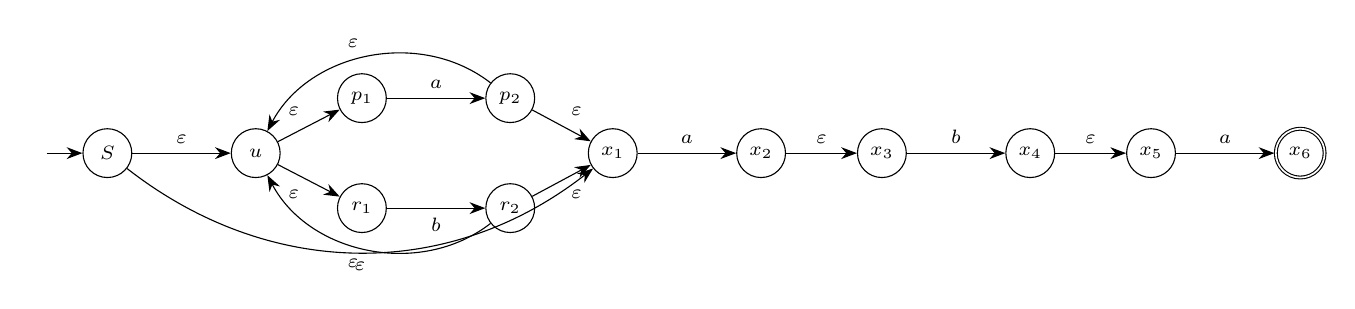
\begin{tikzpicture}[node distance=1.25cm,every state/.style={minimum size=0.62cm,inner sep=0pt,font=\scriptsize},every edge/.append style={font=\scriptsize}]
\node[state,initial,initial text=] (S) {$S$};
\node[state,right=of S] (u) {$u$};
\node[state,above right=0.25cm and 0.9cm of u] (p1) {$p_1$};
\node[state,right=of p1] (p2) {$p_2$};
\node[state,below right=0.25cm and 0.9cm of u] (r1) {$r_1$};
\node[state,right=of r1] (r2) {$r_2$};
\node[state,right=3.9cm of u] (x1) {$x_1$};
\node[state,right=of x1] (x2) {$x_2$};
\node[state,right=0.9cm of x2] (x3) {$x_3$};
\node[state,right=of x3] (x4) {$x_4$};
\node[state,right=0.9cm of x4] (x5) {$x_5$};
\node[state,accepting,right=of x5] (x6) {$x_6$};
\path[->] (S) edge node {$\eps$} (u) (u) edge node {$\eps$} (p1) (u) edge node[swap] {$\eps$} (r1)
 (p1) edge node {$a$} (p2) (r1) edge node[swap] {$b$} (r2)
 (p2) edge[bend right=50] node[swap] {$\eps$} (u) (r2) edge[bend left=50] node {$\eps$} (u)
 (p2) edge node {$\eps$} (x1) (r2) edge node[swap] {$\eps$} (x1) (S) edge[bend right=38] node[swap] {$\eps$} (x1)
 (x1) edge node {$a$} (x2) (x2) edge node {$\eps$} (x3) (x3) edge node {$b$} (x4) (x4) edge node {$\eps$} (x5) (x5) edge node {$a$} (x6);
\end{tikzpicture}
\end{center}
\ansh{Check.} $aba$: $S\xrightarrow{\eps}x_1\xrightarrow{a}\xrightarrow{\eps}\xrightarrow{b}\xrightarrow{\eps}\xrightarrow{a}x_6$ accept;
$baba$: one loop through $r_1\to r_2$, then $\to x_1$ and $aba$ --- accept. $ab$ never reaches $x_6$ --- reject.
(Simplified equivalent NFA: $s\xrightarrow{a,b}s$, $s\xrightarrow{a}1\xrightarrow{b}2\xrightarrow{a}3$, accept 3.)
\end{examq}

\begin{examq}{State elimination (2022-23 Q4(c) type)}{10 marks}
Find a regular expression for the DFA over $\{0,1\}$ with states $E$ (start, accepting) and $O$, where 0 loops on both states and 1 swaps them.
\tcblower
\ansh{Step 1 (GNFA).} New start $s\xrightarrow{\eps}E$, new accept $E\xrightarrow{\eps}f$. Labels: $E\to E:0$, $E\to O:1$, $O\to O:0$, $O\to E:1$.\\
\ansh{Step 2 (rip $O$).} Only path through $O$: $E\to O\to E$, label $1\,0^*\,1$. New loop on $E$: $R(E,E)=0\cup10^*1$.\\
\ansh{Step 3 (rip $E$).} $R(s,f)=\eps\,(0\cup10^*1)^*\,\eps$.\\
\ansh{Answer.} $(0\cup10^*1)^*$ = strings with an even number of 1s. Check: $11$, $0101$ in; $1$, $0111$ out.
\end{examq}

\begin{recipe}[Short theory answers (2--12 marks each) --- write these sentences]
\begin{itemize}
\item \textbf{$\emptyset^*=\{\eps\}$} (2022-23 Q3(c), 2021-22 Q3(a)): $A^*$ includes the concatenation of \emph{zero} strings, $\eps$, for any
$A$; one or more pieces would need a string from $\emptyset$, impossible.
\item \textbf{Swap accept states} (2017-18 Q2(a), 2021-22 Q1(c), 2022-23 Q3(b)): works for a \emph{complete} DFA (one run per string, so it
ends in $F$ or not). Fails without a dead state, and fails for NFAs: $q_0\xrightarrow{a}q_0,\ q_0\xrightarrow{a}q_1$, $F=\{q_1\}$ accepts $a^+$;
swapped it accepts $a^*$, not $\{\eps\}$.
\item \textbf{Star without a new start state} (2023-24 Q3(b)): $N_1$ for $a^*b$ ($q_1\xrightarrow{a}q_1$, $q_1\xrightarrow{b}q_2$). Making $q_1$
accepting accepts $a\notin(a^*b)^*$. The new start state has no incoming edges, so a run cannot stop there half-way.
\item \textbf{Concatenation with $\emptyset$} (2023-24 Q1(c)): the NFA for $\emptyset$ has no accepting state, so the concatenation NFA has
$F=\emptyset$ and accepts nothing: $L\circ\emptyset=\emptyset$.
\item \textbf{Evaluate} (2020 Q3(a)): $\emptyset^*\emptyset^*\emptyset^*\emptyset^*=\{\eps\}$; $\emptyset^*\cup\{\eps\}=\{\eps\}$;
$(\emptyset^*\cup1)\{0,1\}=\{0,1,10,11\}$; $(11)^*\emptyset(00)^*=\emptyset$; $(\emptyset^*\cup0)\{0,1,11\}=\{0,1,11,00,01,011\}$.
\item \textbf{Simplify} (2019-20 Q2(b)): $\emptyset^*\cup a^*\cup b^*\cup(a\cup b)^*=(a\cup b)^*$; $((a^*b^*)^*(b^*a^*)^*)^*=(a\cup b)^*$;
$(a^*b)^*\cup(b^*a)^*=(a\cup b)^*$ (every non-empty string ends in $b$ or in $a$).
\item \textbf{Describe} $(1+\eps)(00^*1)^*0^*$ (2020 Q4(a)): all binary strings with no two consecutive 1s.
\item \textbf{Finite or infinite} (2021-22 Q2(c)): $L_1^*\circ L_2^*$ infinite ($L_1^*$ is infinite and $\eps\in L_2^*$);
$L_1\circ(L_1\cup L_2)$ finite (at most $3\times6$ strings); $L_2\circ L_3$ infinite ($L_3$ is infinite, $L_2\ne\emptyset$).
\end{itemize}
\end{recipe}

% ------------------------------------------------------------------ 5
\section{Pumping lemma (regular)}\markboth{5 Regular pumping lemma}{}
\asked{9 questions. Prove non-regular (2023-24 Q4(c) $a^{n!}$, 2019-20 Q4(c)); criticise an argument (2017-18 Q3(b), 2020 Q1(b),
2021-22 Q1(d), 2019-20 Q1(a)); pumping lengths (2022-23 Q2(b)); why $|xy|\le p$ (2023-24 Q2(a)); why only negative (2021-22 Q4(a)).
All answered in the Proofs PDF, Section 4.}
\begin{recipe}[Recipe --- the five sentences of every non-regularity proof]
\begin{enumerate}
\item ``Assume, for contradiction, that $L$ is regular. Let $p$ be its pumping length.''
\item ``Choose $s=\dots\in L$'' --- written with $p$; check $s\in L$ and $|s|\ge p$. Put a block of $p$ equal symbols first.
\item ``Let $s=xyz$ be \emph{any} split with $|y|>0$ and $|xy|\le p$. Since the first $p$ symbols are \dots, $y=\dots^k$ with $1\le k\le p$.''
\item ``Take $i=\dots$; then $xy^iz=\dots\notin L$ because \dots''
\item ``This contradicts the pumping lemma. Hence $L$ is not regular.''
\end{enumerate}
\textbf{For criticism questions} check: is $s$ in $L$? is $|s|\ge p$? did they choose $y$ themselves? did they claim ``for all $i$''? did
they try to prove a language \emph{regular} with the lemma? (Each is an error.)
\end{recipe}

\begin{examq}{2019-20 Q4(c)}{15 marks}
Use the pumping lemma to prove that $L=\{a^{2n}b^{3n}a^n\mid n\ge0\}$ is not regular.
\tcblower
Assume, for contradiction, that $L$ is regular, and let $p$ be its pumping length.\\
Choose $s=a^{2p}b^{3p}a^{p}$. It is in $L$ (take $n=p$) and $|s|=6p\ge p$.\\
Let $s=xyz$ be any split with $|y|>0$ and $|xy|\le p$. The first $2p\ge p$ symbols of $s$ are $a$'s, so $x$ and $y$ lie in the first block:
$y=a^k$ with $1\le k\le p$.\\
Take $i=2$: $xy^2z=a^{2p+k}b^{3p}a^{p}$. If this were in $L$, the $b$-block $b^{3p}$ would force $n=p$, so the first block would have to be
$a^{2p}$; but it is $a^{2p+k}$ with $k\ge1$. Hence $xy^2z\notin L$.\\
This contradicts the pumping lemma. Therefore $L$ is not regular. $\blacksquare$
\end{examq}

\begin{examq}{2023-24 Q4(c)}{13 marks}
Show that $L=\{a^{n!}\mid n\ge1\}$ is not regular.
\tcblower
Assume $L$ is regular with pumping length $p$. Let $m=\max(p,2)$ and choose $s=a^{m!}\in L$; $|s|=m!\ge m\ge p$.
Any split with $|y|>0$, $|xy|\le p$ has $y=a^k$, $1\le k\le p\le m$. Take $i=2$: $|xy^2z|=m!+k$, and
$m!<m!+k\le m!+m<m!+m\cdot m!=(m+1)!$. So $m!+k$ lies strictly between two consecutive factorials and is not a factorial: $xy^2z\notin L$.
Contradiction; $L$ is not regular. $\blacksquare$
\end{examq}

\begin{trap}\TRAP Never ``let $p=5$''; never pick $x,y,z$; never write ``$xy^iz\notin L$ for all $i$''. A fixed string like $00011000$ is
worthless (it does not depend on $p$). The pumping lemma can never show a language \emph{is} regular. If $p$ might not be prime, do not
choose $a^p$ for the primes --- choose a prime $q>p$.\end{trap}

% ------------------------------------------------------------------ 6
\section{Context-free grammars: design and ambiguity}\markboth{6 CFG}{}
\asked{15 questions. Design with the design idea (2022-23 Q5, 2021-22 Q2(d), 2020 Q5, 2019-20 Q5, 2017-18 Q5); grammar for an inherently
ambiguous language and its ambiguity (2023-24 Q5, 2022-23 Q6, 2020 Q6); is this grammar ambiguous / inherently ambiguous (2021-22 Q6, 2019-20 Q6,
2017-18 Q6); why ``context-free'' (2023-24 Q3(c), 2021-22 Q1(e)).}
\begin{recipe}[Recipe --- designing a CFG]
\begin{enumerate}
\item Split the language into cases joined by \textbf{union} ($S\to S_1\mid S_2$) or pieces joined by \textbf{concatenation} ($S\to S_1S_2$).
\item Matched counts: \textbf{wrap} from the outside in, $X\to aXb\mid\eps$ (nested matching: outer $a$ with outer $b$).
Free part: $C\to cC\mid\eps$. ``At least one extra'': $A\to aA\mid a$.
\item Write the idea in words before the rules; then derive one string from each case.
\item \textbf{Ambiguity:} one string, two leftmost derivations (or two parse trees). That proves the grammar ambiguous.
\end{enumerate}
\textbf{Ready answers:} balanced parentheses $S\to(S)S\mid\eps$; equal 0s and 1s $S\to0S1S\mid1S0S\mid\eps$; at least two 1s
$S\to A1A1A,\ A\to0A\mid1A\mid\eps$; at least one 0 and one 1 $S\to A0A1A\mid A1A0A,\ A\to0A\mid1A\mid\eps$ (all checked by program).
\end{recipe}

\begin{examq}{2021-22 Q2(d)}{15 marks}
Design a context-free grammar for $\{a^ib^jc^k\mid i\ne j+k,\ i,j,k\ge0\}$. Merely putting forth the production rules shall not suffice. You need
to explain your design idea first.
\tcblower
\ansh{Design idea.} If $i=j+k$, every $c$ can be matched with an $a$ from the outside in ($a\dots c$), and then every $b$ with an $a$
($a\dots b$): $a^k\,(a^jb^j)\,c^k$. So $i\ne j+k$ means the matching leaves something over. Three cases:
\begin{enumerate}
\item $i>j+k$: after matching, at least one $a$ is left in the middle.
\item $k\le i<j+k$: all $c$'s are matched by $a$'s, the remaining $a$'s are matched by $b$'s, and at least one $b$ is left.
\item $i<k$: all $a$'s are matched by $c$'s, and the middle is $b^j$ followed by at least one unmatched $c$.
\end{enumerate}
\ansh{Grammar.}
\[\begin{aligned}
S&\to X\mid Y\mid W\\
X&\to aXc\mid P, & P&\to aPb\mid A, & A&\to aA\mid a &&\text{(case 1: } a^k\,a^t\,a^{e}\,b^t\,c^k,\ e\ge1)\\
Y&\to aYc\mid Q, & Q&\to aQb\mid B, & B&\to bB\mid b &&\text{(case 2: } a^k\,a^t\,b^t\,b^{e}\,c^k,\ e\ge1)\\
W&\to aWc\mid U, & U&\to bU\mid C, & C&\to cC\mid c &&\text{(case 3: } a^i\,b^j\,c^{e}\,c^i,\ e\ge1)
\end{aligned}\]
\ansh{Why it is correct.} Each case produces $a^*b^*c^*$ with the stated inequality ($i=j+k+e$, $j=t+e$ with $i=k+t$, or $k=i+e$), and every
string with $i\ne j+k$ falls in case 1 ($i>j+k$), case 2 ($i<j+k$, $i\ge k$) or case 3 ($i<k$).\\
\ansh{Derivations.} $aaab$ ($i=3>1$): $S\Rightarrow X\Rightarrow P\Rightarrow aPb\Rightarrow aAb\Rightarrow aaAb\Rightarrow aaab$.
$abcc$ ($i=1<3$, $i<k$): $S\Rightarrow W\Rightarrow aWc\Rightarrow aUc\Rightarrow abUc\Rightarrow abCc\Rightarrow abcc$.
(Checked by program against the definition on all strings up to length 9.)
\end{examq}

\begin{examq}{2023-24 Q5 (also 2021-22 Q6, 2019-20 Q6)}{15 marks}
Design a CFG for $\{a^ib^jc^k\mid i=j\text{ or }i=k;\ i,j,k\ge1\}$ and show that it is ambiguous.
\tcblower
\ansh{Design idea.} Union of two cases. $i=j$: match $a$ with $b$ ($A\to aAb\mid ab$), then any $c^m$, $m\ge1$. $i=k$: match the outer $a$ with
the outer $c$ ($C\to aCc\mid aDc$), with $b^j$, $j\ge1$, in the middle.
\[S\to AB\mid C,\qquad A\to aAb\mid ab,\quad B\to cB\mid c,\qquad C\to aCc\mid aDc,\quad D\to bD\mid b.\]
\ansh{Ambiguity.} $abc$ has $i=j=k=1$, so it is in both cases. Two leftmost derivations:
\[S\Rightarrow AB\Rightarrow abB\Rightarrow abc,\qquad\qquad S\Rightarrow C\Rightarrow aDc\Rightarrow abc.\]
They start with different rules, so they give two different parse trees (root children $A\,B$ versus $C$). Hence the grammar is ambiguous.
In fact every grammar for this language is ambiguous (it is \emph{inherently ambiguous}): the strings $a^nb^nc^n$ must be generated by both
mechanisms. (Same answer for $\{a^nb^nc^md^m\}\cup\{a^nb^mc^md^n\}$: $S\to AB\mid C$, $A\to aAb\mid ab$, $B\to cBd\mid cd$, $C\to aCd\mid aDd$,
$D\to bDc\mid bc$; $abcd$ has two derivations.)
\end{examq}

\begin{trap}\TRAP A leftmost and a rightmost derivation of the same tree do \emph{not} show ambiguity --- you need two different trees.
``Ambiguous'' is about a grammar; ``inherently ambiguous'' is about a language (every grammar for it is ambiguous). For
$E\to E+E\mid E\times E\mid(E)\mid a$ (2017-18 Q6) use $a+a\times a$ and fix it with $E\to E+T\mid T,\ T\to T\times F\mid F,\ F\to(E)\mid a$.
\textbf{Why ``context-free'':} a variable is rewritten by $A\to\gamma$ regardless of the symbols around it (its context); a context-sensitive
rule $\alpha A\beta\to\alpha\gamma\beta$ may rewrite $A$ only between $\alpha$ and $\beta$.\end{trap}

% ================================================================== PART B
\clearpage
\section*{Part B --- Atif Sir}\addcontentsline{toc}{section}{Part B --- Atif Sir}

% ------------------------------------------------------------------ 7
\section{CNF and the CYK algorithm}\markboth{7 CNF and CYK}{}
\asked{7 questions. CYK with the table (2023-24 Q6, 2022-23 Q7, 2020 Q7, 2019-20 Q7, 2017-18 Q7(b)) --- almost every paper; convert to CNF
(2021-22 Q5, 2017-18 Q7(a)).}
\begin{recipe}[Recipe --- CYK]
Let $w=a_1\cdots a_n$; $X_{ij}$ = set of variables that derive $a_i\cdots a_j$.
\begin{enumerate}
\item Bottom row: $X_{ii}=\{A\mid A\to a_i\}$.
\item Row of length $\ell$: $X_{ij}=\{A\mid A\to BC,\ B\in X_{ik},\ C\in X_{k+1,j}\text{ for some }i\le k<j\}$ --- try \emph{every} split $k$.
\item $w\in L(G)\iff S\in X_{1n}$. Draw the triangle (bottom row = single symbols), show at least the computation for the top cell.
\end{enumerate}
\textbf{CNF order:} remove $\eps$-rules (nullable variables) $\to$ unit rules $\to$ useless symbols $\to$ terminals in long bodies ($U_a\to a$)
$\to$ break bodies longer than 2.
\end{recipe}

\begin{examq}{2022-23 Q7}{15 marks}
For the CNF grammar $S\to AB\mid AY\mid YA\mid1$, $A\to ZA\mid YA\mid0\mid1$, $B\to YA$, $Z\to0$, $Y\to1$, use the CYK algorithm to determine
whether $0100\in L(G)$. Show the table.
\tcblower
\ansh{Row 1 (single symbols).} $0$: $A\to0$, $Z\to0$ $\Rightarrow\{A,Z\}$. $1$: $S\to1$, $A\to1$, $Y\to1$ $\Rightarrow\{A,S,Y\}$.\\
\ansh{Row 2.} $X_{12}$ (``01''): $\{A,Z\}\times\{A,S,Y\}$ contains $ZA$ ($A\to ZA$) and $AY$ ($S\to AY$) $\Rightarrow\{A,S\}$.
$X_{23}$ (``10''): $\{A,S,Y\}\times\{A,Z\}$ contains $YA$ ($A,B,S\to YA$) $\Rightarrow\{A,B,S\}$.
$X_{34}$ (``00''): $\{A,Z\}\times\{A,Z\}$ contains $ZA$ $\Rightarrow\{A\}$.\\
\ansh{Row 3.} $X_{13}$: splits $X_{11}X_{23}$ gives $ZA\to A$, $AB\to S$; so $\{A,S\}$. $X_{24}$: split $X_{22}X_{34}$ gives $YA\to A,B,S$; so $\{A,B,S\}$.\\
\ansh{Row 4.} $X_{14}$: split $k=1$: $X_{11}\times X_{24}=\{A,Z\}\times\{A,B,S\}$ gives $AB$ ($S$) and $ZA$ ($A$) $\Rightarrow\{A,S\}$.
\begin{center}\small
\begin{tabular}{c|cccc}
$\ell=4$ & $\{A,S\}$ & & & \\
$\ell=3$ & $\{A,S\}$ & $\{A,B,S\}$ & & \\
$\ell=2$ & $\{A,S\}$ & $\{A,B,S\}$ & $\{A\}$ & \\
$\ell=1$ & $\{A,Z\}$ & $\{A,S,Y\}$ & $\{A,Z\}$ & $\{A,Z\}$\\\hline
$w$ & $0$ & $1$ & $0$ & $0$
\end{tabular}
\end{center}
\ansh{Conclusion.} $S\in X_{14}$, so $0100\in L(G)$ (e.g.\ $S\Rightarrow AB$ with $A\Rightarrow0$ and $B\Rightarrow100$).
(Here $A$ derives every non-empty string and $L(G)$ = all strings containing at least one 1 --- checked by program.)
\end{examq}

\begin{examq}{2021-22 Q5}{15 marks}
Convert $S\to A1A\mid B$, $A\to0A\mid1A\mid\eps$, $B\to1$ to Chomsky normal form, showing the steps.
\tcblower
\ansh{Step 1 --- $\eps$-rules.} Nullable: $A$. Add every version with $A$ deleted, drop $A\to\eps$:
$S\to A1A\mid1A\mid A1\mid1\mid B$, $A\to0A\mid1A\mid0\mid1$, $B\to1$.\\
\ansh{Step 2 --- unit rules.} $S\to B$ is replaced by $B$'s body: $S\to1$ (already there).\\
\ansh{Step 3 --- useless symbols.} $B$ is no longer reachable from $S$: drop it.
$S\to A1A\mid1A\mid A1\mid1$, $A\to0A\mid1A\mid0\mid1$.\\
\ansh{Step 4 --- terminals in long bodies.} $U\to0$, $V\to1$: $S\to AVA\mid VA\mid AV\mid1$, $A\to UA\mid VA\mid0\mid1$.\\
\ansh{Step 5 --- long bodies.} $S\to AVA$ becomes $S\to AD$, $D\to VA$.\\
\ansh{CNF.} $S\to AD\mid VA\mid AV\mid1$,\ $D\to VA$,\ $A\to UA\mid VA\mid0\mid1$,\ $U\to0$,\ $V\to1$.
(The language is all strings with at least one 1; the CNF grammar and the original agree on all strings up to length 7.)
\end{examq}

\begin{trap}\TRAP In CYK try every split, not only the first one. A cell can be empty --- write $\emptyset$. Remove $\eps$-rules \emph{before}
unit rules, and generating symbols \emph{before} reachable ones. Keep $S\to\eps$ only if $\eps\in L$.\end{trap}

% ------------------------------------------------------------------ 8
\section{Pushdown automata and the CFL pumping lemma}\markboth{8 PDA}{}
\asked{10 questions. Design a PDA with its transition diagram in \emph{every} paper: $\{a^nb^mc^md^n\}$ (2023-24 Q8), $\{a^ib^jc^k\mid i=j\text{ or }
i=k\}$ (2022-23 Q8, 2020 Q8), ARITH (2021-22 Q7, 2019-20 Q8), $\{a^nb^nc^md^m\}$ (2017-18 Q8). Also: final state = empty stack (2019-20 Q10(a));
give a non-CFL and prove it (2023-24 Q7, 2021-22 Q8); state and prove the CFL pumping lemma (2022-23 Q9) --- proofs in the Proofs PDF, 7--8.}
\begin{recipe}[Recipe --- designing a PDA (Atif's notation: $a,X/\gamma$ = read $a$, pop $X$, push $\gamma$, leftmost on top)]
\begin{enumerate}
\item \textbf{Stack strategy} in one sentence: what one stack symbol stands for.
\item Start with $Z_0$ on the stack; seeing $Z_0$ on top means ``everything matched''.
\item One state per \textbf{phase} of the input ($a$-part, $b$-part, \dots). Separate arcs for the \emph{first} symbol of a block when the
block must be non-empty.
\item ``Or'' in the language $\Rightarrow$ an $\eps$-guess at the start. Missing transition = that branch dies.
\item Say how it accepts (final state or empty stack), draw the diagram, give the 7-tuple, trace one accepted and one rejected string as IDs.
\end{enumerate}
\textbf{CFG $\to$ PDA (empty stack):} one state $q$; $\delta(q,\eps,A)\ni(q,\beta)$ for each rule $A\to\beta$; $\delta(q,a,a)=\{(q,\eps)\}$; start stack $S$.
\end{recipe}

\begin{examq}{2023-24 Q8}{15 marks}
Design a PDA for $\{a^nb^mc^md^n\mid n\ge1,\ m\ge1\}$. Draw its transition diagram.
\tcblower
\ansh{Idea.} Push an $A$ for every $a$ and a $B$ for every $b$; pop a $B$ for every $c$, then an $A$ for every $d$. The $B$'s sit above the
$A$'s, so the $c$'s are matched with the $b$'s and the $d$'s with the $a$'s (nested). Reading $c$ with $A$ on top (too many $c$'s) or $d$ with
$B$ on top (too few $c$'s) has no move, so that run dies. Accept by final state when $Z_0$ is back on top.
\[P=(\{q_0,\dots,q_5\},\{a,b,c,d\},\{A,B,Z_0\},\delta,q_0,Z_0,\{q_5\})\]
\begin{center}
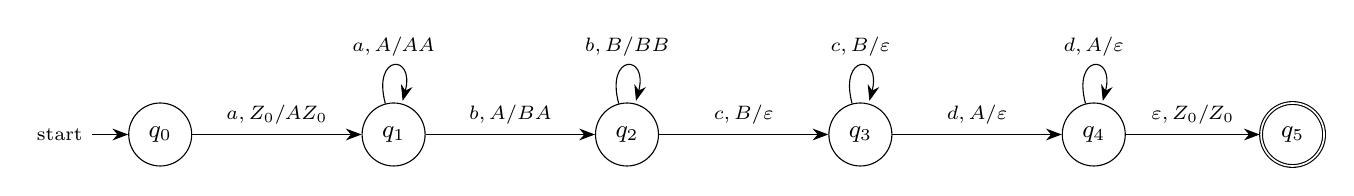
\begin{tikzpicture}[node distance=2.15cm,every edge/.append style={font=\scriptsize}]
\node[state,initial] (0) {$q_0$};
\node[state,right=of 0] (1) {$q_1$};
\node[state,right=of 1] (2) {$q_2$};
\node[state,right=of 2] (3) {$q_3$};
\node[state,right=of 3] (4) {$q_4$};
\node[state,accepting,right=1.7cm of 4] (5) {$q_5$};
\path[->] (0) edge node {$a,Z_0/AZ_0$} (1) (1) edge[loop above] node {$a,A/AA$} ()
 (1) edge node {$b,A/BA$} (2) (2) edge[loop above] node {$b,B/BB$} ()
 (2) edge node {$c,B/\eps$} (3) (3) edge[loop above] node {$c,B/\eps$} ()
 (3) edge node {$d,A/\eps$} (4) (4) edge[loop above] node {$d,A/\eps$} ()
 (4) edge node {$\eps,Z_0/Z_0$} (5);
\end{tikzpicture}
\end{center}
\ansh{Accepted: $aabcdd$.} $(q_0,aabcdd,Z_0)\vdash(q_1,abcdd,AZ_0)\vdash(q_1,bcdd,AAZ_0)\vdash(q_2,cdd,BAAZ_0)\vdash(q_3,dd,AAZ_0)$
$\vdash(q_4,d,AZ_0)\vdash(q_4,\eps,Z_0)\vdash(q_5,\eps,Z_0)$ --- accept.\\
\ansh{Rejected: $aabccd$.} $\dots\vdash(q_2,ccd,BAAZ_0)\vdash(q_3,cd,AAZ_0)$: reading $c$ with $A$ on top has no move --- the only run dies, reject.
$n,m\ge1$ is enforced by the separate first-$a$ and first-$b$ arcs. (Checked by program on all strings up to length 9.)
\end{examq}

\begin{examq}{2021-22 Q7 and 2019-20 Q8}{15 marks}
Construct a PDA for ARITH, the legal arithmetic expressions over $\{a,+,*,(,)\}$ (valid: $a+a*a$, $((a+a)*(a+a))+(a)$; invalid: $aa*a$, $a++a$,
$+a$, $(a+a))$). Give its transition diagram.
\tcblower
\ansh{Idea.} ARITH is generated by the (unambiguous) grammar $E\to E+T\mid T$, $T\to T*F\mid F$, $F\to(E)\mid a$. Convert it to a PDA that
simulates leftmost derivations: expand the variable on top of the stack, match terminals with the input. Accept by empty stack.
\[P=(\{q\},\{a,+,*,(,)\},\{E,T,F,a,+,*,(,)\},\delta,q,E)\]
\begin{center}
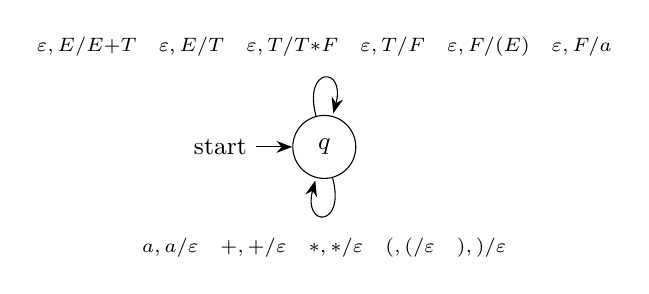
\begin{tikzpicture}
\node[state,initial] (q) {$q$};
\path[->] (q) edge[loop above] () (q) edge[loop below] ();
\node[above=0.62cm of q,font=\scriptsize,align=center] {$\eps,E/E{+}T\quad \eps,E/T\quad \eps,T/T{*}F\quad \eps,T/F\quad \eps,F/\mathtt{(}E\mathtt{)}\quad \eps,F/a$};
\node[below=0.62cm of q,font=\scriptsize,align=center] {$a,a/\eps\quad {+},{+}/\eps\quad {*},{*}/\eps\quad \mathtt{(},\mathtt{(}/\eps\quad \mathtt{)},\mathtt{)}/\eps$};
\end{tikzpicture}
\end{center}
\ansh{Accepted: $a+a*a$.} $(q,a{+}a{*}a,E)\vdash(q,a{+}a{*}a,E{+}T)\vdash(q,a{+}a{*}a,T{+}T)\vdash(q,a{+}a{*}a,F{+}T)\vdash(q,a{+}a{*}a,a{+}T)$
$\vdash(q,{+}a{*}a,{+}T)\vdash(q,a{*}a,T)\vdash(q,a{*}a,T{*}F)\vdash(q,a{*}a,F{*}F)\vdash(q,a{*}a,a{*}F)\vdash(q,{*}a,{*}F)\vdash(q,a,F)\vdash(q,a,a)\vdash(q,\eps,\eps)$ --- accept.\\
\ansh{Rejected: $a{+}{+}a$.} After matching $a+$ the stack holds $T$ (or more); every expansion of $T$ puts $a$ or $($ on top, never $+$, so
the second $+$ can never be matched: every run dies. (For acceptance by final state, add the empty-stack $\to$ final-state construction.)
\end{examq}

\begin{examq}{2022-23 Q8 and 2020 Q8}{15 marks}
Design a PDA for $\{a^ib^jc^k\mid i=j\text{ or }i=k\}$.
\tcblower
\ansh{Idea.} Guess at the start which equality holds. Branch $i=j$: push $A$ per $a$, pop per $b$, back at $Z$ allow any $c$'s.
Branch $i=k$: push $A$ per $a$, skip the $b$'s, pop per $c$. Accept by final state ($p_2$, $r_3$).
\begin{center}\small
\begin{tabular}{@{}ll@{}}
start: & $\delta(q_0,\eps,Z)=\{(p_0,Z),(r_0,Z)\}$\\
$i=j$: & $(p_0,a,Z/AZ)$, $(p_0,a,A/AA)$, $(p_0\to p_1,b,A/\eps)$, $(p_1,b,A/\eps)$, $(p_0\to p_2,\eps,Z/Z)$, $(p_1\to p_2,\eps,Z/Z)$, $(p_2,c,Z/Z)$\\
$i=k$: & $(r_0,a,Z/AZ)$, $(r_0,a,A/AA)$, $(r_0\to r_1,\eps,X/X)$, $(r_1,b,X/X)$, $(r_1\to r_2,c,A/\eps)$, $(r_2,c,A/\eps)$,\\
 & $(r_1\to r_3,\eps,Z/Z)$, $(r_2\to r_3,\eps,Z/Z)$\qquad ($X\in\{A,Z\}$)
\end{tabular}
\end{center}
\ansh{Trace $aabcc$ (branch $i=k$).} $(q_0,aabcc,Z)\vdash(r_0,aabcc,Z)\vdash(r_0,abcc,AZ)\vdash(r_0,bcc,AAZ)\vdash(r_1,bcc,AAZ)\vdash(r_1,cc,AAZ)$
$\vdash(r_2,c,AZ)\vdash(r_2,\eps,Z)\vdash(r_3,\eps,Z)$ --- accept. $aab$: branch 1 is left with $A$ on top, branch 2 has no $c$ --- reject.
(2017-18 Q8, $\{a^nb^nc^md^m\}$: push per $a$, pop per $b$, then push per $c$, pop per $d$, with first-symbol arcs for $n,m\ge1$.)
\end{examq}

\begin{examq}{2023-24 Q7 and 2021-22 Q8}{15 marks}
Give an example of a language that is not context-free, and prove it using the pumping lemma for CFLs.
\tcblower
\ansh{Example.} $L=\{0^n1^n2^n\mid n\ge1\}$.\\
\ansh{Lemma (HMU).} If $L$ is a CFL there is $n$ such that every $z\in L$, $|z|\ge n$, is $z=uvwxy$ with $|vwx|\le n$, $vx\ne\eps$ and
$uv^iwx^iy\in L$ for all $i\ge0$.\\
\ansh{Proof.} Assume $L$ is a CFL with constant $n$. Choose $z=0^n1^n2^n\in L$, $|z|=3n\ge n$. Let $z=uvwxy$ be any split with $|vwx|\le n$,
$vx\ne\eps$. Since $|vwx|\le n$, $vwx$ cannot contain both a 0 and a 2 (all $n$ 1s lie between them).
(a) If $v$ or $x$ contains two different symbols, $uv^2wx^2y$ has them out of order, so it is not in $0^*1^*2^*$.
(b) Otherwise, if $vwx$ has no 2, then $uwy$ ($i=0$) still has $n$ 2s but fewer 0s or fewer 1s; if $vwx$ has no 0, $uwy$ has $n$ 0s but
fewer 1s or 2s. In every case some $uv^iwx^iy\notin L$, contradicting the lemma. Hence $L$ is not context-free. $\blacksquare$
\end{examq}

\begin{trap}\TRAP Say what each stack symbol means. Show the IDs $(q,\text{remaining input},\text{stack})$ --- the trace earns marks.
A PDA needs nondeterminism for ``or'' languages and for $ww^R$; say so. In the CFL lemma you choose $z$ and $i$ only; pump $v$ and $x$
\emph{together}; cover every placement of $vwx$.\end{trap}

% ------------------------------------------------------------------ 9
\section{Turing machine design on $w_1cw_2c$}\markboth{9 TM design}{}
\asked{6 questions, one in every paper, all on the same pattern: AND (2019-20 Q9), OR (2017-18 Q9), XOR (2020 Q9), equality test
(2023-24 Q9), NOT after $c$ (2022-23 Q10), signed magnitude $\to$ 2's complement (2021-22 Q9). Multiple tracks and storage in the state are allowed.}
\begin{recipe}[Recipe --- a bit-by-bit TM]
\begin{enumerate}
\item \textbf{Algorithm in words:} take the leftmost unmarked bit of $w_1$, remember it in the state, mark it; walk to the leftmost unmarked bit
of $w_2$, combine, mark it; walk past the second $c$ to the first blank and write the result bit; return to the left end; repeat.
\item \textbf{Marking:} $0\mapsto X$, $1\mapsto Y$ (or a check mark on a second track). \textbf{State storage:} $p_b$, $t_o$ carry a bit.
\item \textbf{Stop:} when the leftmost-unmarked search reaches the first $c$; restore $X\to0$, $Y\to1$ if the output must show $w_1,w_2$.
\item Give the 7-tuple, the transition table (only the moves that occur), and a sweep-by-sweep trace of a short input.
\end{enumerate}
\end{recipe}

\begin{examq}{2019-20 Q9}{15 marks}
Design a TM computing the AND of equal-length binary $w_1$ and $w_2$. Initially the tape is $w_1cw_2c$; finish with their AND in binary after
the second $c$.
\tcblower
\ansh{Idea.} Repeat: mark the leftmost unmarked bit $b$ of $w_1$ ($0\to X$, $1\to Y$) and remember it in the state ($p_b$); go past the first
$c$ to the leftmost unmarked bit $b'$ of $w_2$, mark it and remember $o=b\wedge b'$ ($t_o$); go past the second $c$ and the result bits to the
first blank and write $o$; go back to the left end. When the search in $w_1$ meets $c$, every bit is done: restore the marks and halt.
\[M=(\{q_0,p_0,p_1,s_0,s_1,t_0,t_1,u_0,u_1,k,\ell,r,h\},\{0,1,c\},\{0,1,c,X,Y,B\},\delta,q_0,B,\{h\})\]
\begin{center}\small
\begin{tabular}{@{}l|l@{}}
state (meaning) & moves $\delta(\text{state},\text{read})=(\text{state},\text{write},\text{dir})$\\\hline
$q_0$ (find next bit of $w_1$) & $X,Y\to$ same, $R$;\ $0\to(p_0,X,R)$;\ $1\to(p_1,Y,R)$;\ $c\to(\ell,c,L)$\\
$p_b$ (carry $b$ to $w_2$) & $0,1\to$ same, $R$;\ $c\to(s_b,c,R)$\\
$s_b$ (find next bit of $w_2$) & $X,Y\to$ same, $R$;\ $0\to(t_{b\wedge0},X,R)$;\ $1\to(t_{b\wedge1},Y,R)$\\
$t_o$ (go past 2nd $c$) & $0,1\to$ same, $R$;\ $c\to(u_o,c,R)$\\
$u_o$ (write result) & $0,1\to$ same, $R$;\ $B\to(k,o,L)$\\
$k$ (back to left end) & $0,1,c,X,Y\to$ same, $L$;\ $B\to(q_0,B,R)$\\
$\ell$ (done: to left end) & $X,Y,c\to$ same, $L$;\ $B\to(r,B,R)$\\
$r$ (restore) & $X\to(r,0,R)$;\ $Y\to(r,1,R)$;\ $0,1,c\to$ same, $R$;\ $B\to(h,B,R)$
\end{tabular}
\end{center}
\ansh{Trace on $101c110c$} (tape after each round): \quad
$101c110c\ \vdash^*\ Y01cY10c\mathbf1\ \vdash^*\ YX1cYY0c1\mathbf0\ \vdash^*\ YXYcYYXc10\mathbf0\ \vdash^*\ 101c110c100$ (restore, halt).
Round 1: $1\wedge1=1$; round 2: $0\wedge1=0$; round 3: $1\wedge0=0$. Result $100=101\wedge110$. (Checked by program on all equal-length
pairs of length 1--5.)
\end{examq}

\begin{recipe}[The same machine for the other papers --- change only these lines]
\begin{itemize}
\item \textbf{OR (2017-18 Q9, $N_1\#N_2\#$)} / \textbf{XOR (2020 Q9):} in $s_b$ go to $t_{b\vee b'}$ / $t_{b\oplus b'}$.
\item \textbf{Equality (2023-24 Q9):} in $s_b$, if $b'=b$ mark and go back ($k$); if $b'\ne b$ go right past the second $c$ and write 1, halt.
If $q_0$ reaches the first $c$ (all bits matched), go past the second $c$ and write 0, halt.
\item \textbf{NOT after $c$ (2022-23 Q10, tape $wc$):} no second word: from $p_b$ go past $c$ to the first blank, write $1-b$, come back.
\item \textbf{Signed magnitude $\to$ 2's complement (2021-22 Q9, MSB 1):} go to the right end; moving left, copy bits up to and including the
first 1; after that invert every remaining magnitude bit; leave the sign bit 1. (Check: $1\,0110$ ($-6$) $\to$ $1\,1010$.)
\end{itemize}
\end{recipe}

% ------------------------------------------------------------------ 10
\section{Turing-machine variants and simulations}\markboth{10 TM variants}{}
\asked{6 questions, every paper: how a one-tape TM with tracks and state storage simulates a multitape TM (2023-24 Q10, 2019-20 Q10(b)); true/false
on simulations with polynomial cost (2022-23 Q11, 2021-22 Q10, 2020 Q10, 2017-18 Q10).}

\begin{examq}{2023-24 Q10}{15 marks}
What is a multitape TM? Explain how a one-tape TM with multiple tracks and storage in the state can simulate it.
\tcblower
\ansh{Multitape TM.} A finite control with $k$ tapes, each with its own head. Input on tape 1, other tapes blank. One move depends on the
state and all $k$ scanned symbols; it changes state, writes on each tape and moves each head independently ($L$, $R$ or $S$).\\
\ansh{Simulation.} One-tape $N$ uses $2k$ tracks: for each tape of $M$, one track holds its contents and one track holds a single marker $X$
under that tape's head. Example for $k=2$:
\begin{center}\small
\begin{tabular}{l|cccccc}
head 1 & & & $X$ & & &\\
tape 1 & $A_1$ & $A_2$ & $A_3$ & $A_4$ & $\cdots$ &\\
head 2 & & $X$ & & & &\\
tape 2 & $B_1$ & $B_2$ & $B_3$ & $\cdots$ & &
\end{tabular}
\end{center}
$N$'s state stores $M$'s state and a count of how many head markers lie to its left. To simulate one move of $M$:
(1) $N$ sweeps right from the leftmost marker, visiting all $k$ markers and storing the $k$ scanned symbols in its state; now it knows $M$'s move.
(2) It sweeps back, at each marker writes the new symbol on the contents track and moves the marker one cell left/right as $M$ would.
(3) It records $M$'s new state. $N$ accepts when the stored state of $M$ is accepting. So $L(N)=L(M)$.\\
\ansh{Cost.} After $n$ moves the markers are at most $2n$ cells apart, so one simulated move takes $O(n)$ moves and $n$ moves take $O(n^2)$.
\end{examq}

\begin{recipe}[True / false answers (justify in two lines each)]
\begin{itemize}
\item One-tape TM with multiple tracks (and state storage) simulates a multitape TM --- \textbf{True}, $2k$ tracks, $O(n^2)$ time.
\item A DTM simulates $n$ steps of a computer in $p(n)$ steps --- \textbf{True} (if each instruction lengthens a word by at most 1 bit):
$O(n^3)$ multitape, $O(n^6)$ one-tape. Memory is (address, value) pairs on tape 1, at most $O(n^2)$ cells; each instruction costs $O(n^2)$.
\item A DTM (or a computer) simulates $n$ moves of an NTM in $p(n)$ moves --- \textbf{Not known; believed false.} The known method is breadth-first
search of the computation tree: up to $(n+1)m^n$ IDs, exponential. A polynomial simulation would give $\P=\NP$.
\end{itemize}
\end{recipe}

% ------------------------------------------------------------------ 11
\section{Undecidability}\markboth{11 Undecidability}{}
\asked{7 questions, every paper: $L_d$ is not RE (2022-23 Q12, 2017-18 Q11); the halting problem is RE but not recursive (2019-20 Q12,
2023-24 Q11, 2021-22 Q11); definitions and one example per class (2020 Q11, 2019-20 Q11). Notation as in Atif Sir's slides (Hopcroft).}
\begin{recipe}[Recipe --- the three proofs to know]
\textbf{$L_d$ not RE} (diagonalisation): if $L_d=L(M_i)$, ask whether $w_i\in L_d$ --- both answers contradict the definition.
\textbf{$L_u$ not recursive:} a decider for $L_u$ gives one for $\overline{L_u}$, which gives a TM for $L_d$ (input $w\mapsto w111w$).
\textbf{Halting not recursive:} a decider for $H$ would decide $L_u$ (``does $M$ halt? if yes, run it''). \textbf{RE:} simulate (universal TM).\\
\textbf{Reduction rule:} if $P_1$ reduces to $P_2$ and $P_1$ is not recursive (not RE), then $P_2$ is not recursive (not RE).
\end{recipe}

\begin{examq}{2019-20 Q12 (also 2023-24 Q11, 2021-22 Q11)}{15 marks}
Define the halting problem. Prove that it is recursively enumerable but not recursive.
\tcblower
\ansh{Definition.} For a TM $M$, $H(M)$ is the set of inputs on which $M$ halts (accepting or not). The halting problem is
$H=\{(M,w)\mid w\in H(M)\}$.\\
\ansh{$H$ is RE.} Build $U_H$ like the universal TM: on input $(M,w)$ simulate $M$ on $w$; if $M$ halts (in any state), accept. If $M$ runs
forever, $U_H$ runs forever, which is allowed. So $L(U_H)=H$ and $H$ is RE.\\
\ansh{$H$ is not recursive.} We use that $L_u=\{(M,w)\mid M\text{ accepts }w\}$ is not recursive. Suppose, for contradiction, that $H$ is
recursive, decided by a TM $D$ that always halts. Then decide $L_u$ as follows. On input $(M,w)$:
(1) run $D$ on $(M,w)$; if $D$ says $M$ does not halt on $w$, reject (a machine that never halts never accepts);
(2) otherwise simulate $M$ on $w$ --- it is guaranteed to halt --- and accept iff it halts in an accepting state.
This procedure always halts and accepts exactly $L_u$, so $L_u$ would be recursive --- a contradiction. Hence $H$ is not recursive.
(We have reduced $L_u$ to $H$.) $\blacksquare$
\end{examq}

\begin{examq}{2022-23 Q12 (also 2017-18 Q11)}{15 marks}
Define the diagonalization language $L_d$ and prove that it is not recursively enumerable.
\tcblower
\ansh{Definition.} Order binary strings $w_1=\eps,w_2=0,w_3=1,w_4=00,\dots$ ($1w_i$ is $i$ in binary). Every TM with input alphabet $\{0,1\}$ has a
binary code ($\delta(q_i,X_j)=(q_k,X_l,D_m)$ coded $0^i10^j10^k10^l10^m$, transitions separated by $11$); $M_i$ is the TM with code $w_i$ (the
TM with no moves if $w_i$ is not a valid code). $L_d=\{w_i\mid w_i\notin L(M_i)\}$ --- the complement of the diagonal of the table
``$M_i$ accepts $w_j$''.\\
\ansh{Proof.} Suppose $L_d=L(M)$ for some TM $M$. Its input alphabet is $\{0,1\}$, so $M=M_i$ for some $i$. If $w_i\in L_d$ then $M_i$
accepts $w_i$, so by definition $w_i\notin L_d$. If $w_i\notin L_d$ then $M_i$ does not accept $w_i$, so by definition $w_i\in L_d$.
Both cases are contradictions, so no TM accepts $L_d$: $L_d$ is not RE. $\blacksquare$
\end{examq}

\begin{recipe}[One example per class (2019-20 Q11, 2020 Q11)]
Regular: $0^*1^*$.\quad CF not regular: $\{0^n1^n\}$.\quad Recursive not CF: $\{0^n1^n2^n\}$ (a marking TM always halts; not CF by the
pumping lemma).\quad RE not recursive: $L_u$ or $H$.\quad Not RE: $L_d$ (or $\overline{L_u}$).\\
RE: $L=L(M)$ for some TM. Recursive: $L=L(M)$ for a TM that halts on every input. If $L$ and $\overline L$ are both RE, $L$ is recursive.
\end{recipe}

% ------------------------------------------------------------------ 12
\section{Complexity: Cook's theorem, NP-completeness, space}\markboth{12 Complexity}{}
\asked{17 questions. Cook's theorem and its clauses in 4 papers (2023-24 Q13, 2022-23 Q13(i), 2021-22 Q12, 2020 Q12(a)); class relationships,
Venn diagram, PSPACE vs NPSPACE in every paper (2023-24 Q12, 2022-23 Q13(ii), 2021-22 Q13, 2020 Q12(b), 2019-20 Q13, 2017-18 Q13);
NP-completeness proofs (2017-18 Q1(b), Q12) and an NP certificate (2020 Q1(a)).}

\begin{examq}{2023-24 Q13}{15 marks}
Explain how Cook's theorem shows that every problem in NP reduces to SAT. An NTM has $\delta(q,t)=\{(q_1,t_1,R),(q_2,t_2,L)\}$; construct its
Boolean-formula rule under Cook's construction when the head is on cell $i$ at step $j$ (not at either end).
\tcblower
\ansh{Cook's theorem: SAT is NP-complete.} SAT $\in\NP$: guess an assignment, evaluate in polynomial time. For any $L\in\NP$ take an NTM
$M$ with at most $p(n)$ moves on every branch. For input $w$ build $F(M,w)$, satisfiable iff some branch accepts; an assignment describes one
branch. Variables: $s(q,j)$ (state $q$ at step $j$), $l_{ij}$ (head on cell $i$ at step $j$), $c(i,j,t)$ (cell $i$ holds $t$ at step $j$),
$u(i,j)$ (cell $i$ unchanged from $j$ to $j+1$), for $0\le i,j\le p(n)$. Seven rule families: (1) exactly one state per step; (2) exactly one
head position; (3) exactly one symbol per cell; (4) unchanged cells keep their symbol; (5) each step follows $\delta$; (6) step 0 is the initial
ID $q_0\,w\,B^{p(n)+1-n}$; (7) the state at step $p(n)$ is accepting. $F(M,w)$ is their AND; the largest family (5) has size
$O(|Q||\Gamma|p(n)^3)$, so $F$ is built in polynomial time and $w\in L\iff F(M,w)$ is satisfiable. So every NP language reduces to SAT.\\
\ansh{The rule.} Here $d_1=R$, $d_2=L$, so the new head positions are $i+1$ and $i-1$:
\[\begin{aligned}\big[s(q,j)\wedge l_{ij}\wedge c(i,j,t)\big]\to\ \bigwedge_{k\ne i}u(k,j)\ \wedge\ \Big[&\big(s(q_1,j{+}1)\wedge l_{(i+1)(j+1)}\wedge c(i,j{+}1,t_1)\big)\\
\vee\ &\big(s(q_2,j{+}1)\wedge l_{(i-1)(j+1)}\wedge c(i,j{+}1,t_2)\big)\Big].\end{aligned}\]
In words: if at step $j$ the state is $q$ and the head reads $t$ on cell $i$, then every other cell is unchanged and at step $j+1$ either
(state $q_1$, cell $i$ holds $t_1$, head on $i+1$) or (state $q_2$, cell $i$ holds $t_2$, head on $i-1$). The $\vee$ is where the satisfying
assignment chooses the branch.
\end{examq}

\begin{examq}{2023-24 Q12, 2022-23 Q13(ii), 2020 Q12(b), 2019-20 Q13}{7--15 marks}
Draw a Venn diagram of P, NP, NP-complete, PSPACE, recursive and RE. What is the relationship between PSPACE and NPSPACE? Justify.
\tcblower
\begin{center}
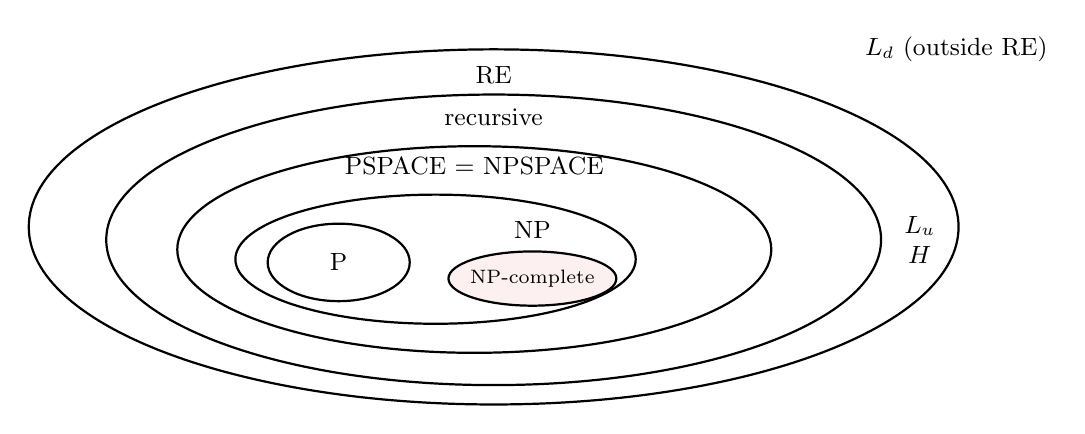
\begin{tikzpicture}[scale=0.82,every node/.style={font=\small}]
\draw[thick] (0,0) ellipse (7.2 and 2.75); \node at (0,2.35) {RE};
\draw[thick] (0,-0.2) ellipse (6 and 2.25); \node at (0,1.7) {recursive};
\draw[thick] (-0.3,-0.35) ellipse (4.6 and 1.6); \node at (-0.3,0.95) {PSPACE $=$ NPSPACE};
\draw[thick] (-0.9,-0.5) ellipse (3.1 and 1.0);  \node at (0.6,-0.05) {NP};
\draw[thick] (-2.4,-0.55) ellipse (1.1 and 0.6); \node at (-2.4,-0.55) {P};
\draw[thick,fill=trapbg] (0.6,-0.8) ellipse (1.3 and 0.42); \node[font=\scriptsize] at (0.6,-0.8) {NP-complete};
\node[align=center] at (6.6,-0.2) {$L_u$\\$H$}; \node[anchor=west] at (5.6,2.75) {$L_d$ (outside RE)};
\end{tikzpicture}
\end{center}
\ansh{Justification.} $\P\subseteq\NP$: a DTM is an NTM with no choices. $\NP\subseteq\PS$: in $T(n)$ moves at most $T(n)+1$ cells are visited,
so $\NP\subseteq\mathrm{NPSPACE}=\PS$. NP-complete problems are in NP and, if $\P\ne\NP$, outside P. Every class here is decided by machines that
always halt (a $p(n)$-space machine can be stopped after $c^{1+p(n)}$ moves), so it lies inside the recursive languages; $L_u$, $H$ are RE but not
recursive; $L_d$ is not RE. Proper inclusions $\P\ne\NP\ne\PS$ are believed, not proved.\\
\ansh{PSPACE $=$ NPSPACE (Savitch).} $\PS\subseteq\mathrm{NPSPACE}$ trivially. Conversely an $f(n)$-space NTM is simulated deterministically
by \textsc{reach}$(I,J,m)$: ``can ID $I$ reach ID $J$ in $\le m$ moves?'', answered by trying every middle ID $K$ and recursing on $(I,K,m/2)$
and $(K,J,m/2)$ one after the other. With $m=c^{1+f(n)}$ the recursion depth is $\log_2 m=O(f(n))$ and each frame is $O(f(n))$ cells, so the
space is $O(f^2(n))$ --- polynomial when $f$ is. Hence PSPACE $=$ NPSPACE.
\end{examq}

\begin{examq}{2017-18 Q12}{15 marks}
Prove that the subgraph-isomorphism problem (does $G_1$ contain a copy of $G_2$ as a subgraph?) is NP-complete.
\tcblower
\ansh{In NP.} Certificate: a one-to-one map $f:V(G_2)\to V(G_1)$. Check in polynomial time that $f$ is one-to-one and that
$(f(u),f(v))\in E(G_1)$ for every edge $(u,v)\in E(G_2)$.\\
\ansh{NP-hard: CLIQUE $\le_p$ SUBISO.} CLIQUE is NP-complete. Map $\langle G,k\rangle$ to $\langle G_1,G_2\rangle=\langle G,K_k\rangle$ ($K_k$ =
complete graph on $k$ vertices, written in $O(k^2)$ time). If $G$ has a $k$-clique $S$, any bijection $V(K_k)\to S$ maps every edge of $K_k$
onto an edge of $G$, so $G$ contains $K_k$. If $K_k$ embeds in $G$ by $f$, the $k$ image vertices are pairwise adjacent, a $k$-clique. So
$\langle G,k\rangle\in$ CLIQUE $\iff\langle G,K_k\rangle\in$ SUBISO.\\
\ansh{Conclusion.} SUBISO is in NP and an NP-complete problem reduces to it in polynomial time; hence it is NP-complete. $\blacksquare$
\end{examq}

\begin{trap}\TRAP Reduce \emph{from} the known NP-complete problem \emph{to} the new one. Prove both directions and say the reduction is polynomial.
A certificate answer (Dominating Set, 2020 Q1(a)) has three parts: what the certificate is, that it is polynomial size, and the polynomial-time
check (every vertex is in $D$ or next to $D$, $|D|\le k$). ``SAT in P $\Rightarrow$ P $=$ NP'' is \textbf{true}; ``NP $\supseteq$ PSPACE'' is
\textbf{not known and believed false}.\end{trap}

\begin{tcolorbox}[colback=white,colframe=navy,boxrule=0.4pt,arc=1pt,left=6pt,right=6pt,top=3pt,bottom=3pt]
\textbf{Last evening before the exam.} (1) Redo the exam answers in Topics 2, 3, 6 (Hakim) and 7, 8, 9 (Atif) on paper without looking ---
these are the design questions that appear every year. (2) Learn the five-sentence pumping proof and the three undecidability proofs by heart.
(3) Read Cook's seven rules and the Venn diagram once more. (4) Skim the short theory answers in Topics 2 and 4.
\end{tcolorbox}

\end{document}
